\chapter{Skalabilitas, Sistem Web Terdistribusi, dan Emerging Web}
\label{ch:skala}

\section*{Tujuan Pembelajaran}
\begin{itemize}
  \item Mengukur penskalaan horizontal sampai satu komponen bersama menjadi
        \textit{bottleneck}, lalu menunjukkan pergeseran
        \textit{bottleneck}-nya dari angka hasil pengukuran.
  \item Merancang rencana kapasitas untuk beban 100 kali lipat yang mencakup
        batas layanan, replikasi, partisi, dan biaya.
  \item Membandingkan manfaat dan biaya tiga teknologi yang sedang tumbuh,
        yaitu mode \textit{offline} Progressive Web App (PWA), \textit{cold
        start} pada \textit{serverless}, dan fitur berbantuan Large Language
        Model (LLM), berdasarkan hasil pengukuran.
\end{itemize}

\section{Pendahuluan}

Bab-bab sebelumnya membangun satu aplikasi lalu mengukurnya di satu mesin.
Pertanyaan yang tersisa justru yang paling sering diajukan: apa yang terjadi
ketika bebannya naik 100 kali lipat? Dua jawaban cepat sama-sama menyesatkan.
Membeli server yang lebih besar ada batasnya, dan memecah aplikasi menjadi
banyak layanan menambah jaringan di antara bagian yang dahulu cukup saling
memanggil.

Bab ini menjawabnya dengan pengukuran. Replika ditambah sampai satu
komponen bersama penuh. Panggilan fungsi dibandingkan dengan panggilan
lewat jaringan. Dua cara membagi data diadu, lalu seluruh angkanya disusun
menjadi satu rencana kapasitas. Bagian akhir membahas teknologi yang sedang
tumbuh, yaitu PWA, WebAssembly, \textit{serverless}, dan LLM, karena
masing-masing memindahkan tempat \textit{latency}, biaya, privasi, dan keamanan
ditentukan.

Referensi utamanya adalah Kleppmann untuk replikasi dan partisi
\cite{kleppmann2017ddia}, Newman untuk batas layanan
\cite{newman2021microservices}, spesifikasi Service Workers dari World Wide
Web Consortium (W3C) \cite{w3c-service-workers}, tinjauan Berkeley tentang
\textit{serverless} \cite{jonas2019serverless}, dan daftar risiko aplikasi
LLM dari Open Worldwide Application Security Project (OWASP)
\cite{owasp-llm-top10}.

\section{Penskalaan Vertikal dan Horizontal}

Penskalaan vertikal berarti memindahkan aplikasi ke mesin yang lebih besar:
core lebih banyak, memori lebih besar, \textit{disk} lebih cepat. Kodenya
tidak berubah sama sekali. Penskalaan horizontal berarti menjalankan beberapa
\textit{copy} aplikasi, disebut replika, di belakang satu penyeimbang beban yang
membagi permintaan di antara mereka.

Analoginya seperti warung dengan satu kasir yang antreannya mengular.
Penskalaan vertikal berarti mengganti kasirnya dengan yang lebih cepat.
Penskalaan horizontal berarti membuka kasir kedua, ketiga, dan seterusnya.
Namun seluruh kasir itu tetap mengambil pesanan dari satu dapur, dan ketika
dapurnya penuh, kasir tambahan hanya memindahkan antrean ke depan dapur.

Penskalaan horizontal punya satu syarat: replika tidak boleh menyimpan
\textit{state} di dalam prosesnya. Sesi pengguna disimpan di luar proses
atau diganti token bertanda tangan seperti pada Bab 10, dan \textit{cache}
di Redis seperti pada Bab 4, sehingga
permintaan mana pun boleh dilayani replika mana pun \cite{twelve-factor}.
Gambar \ref{fig:skala14} memperlihatkan susunan demo bab ini.

\begin{figure}[!htb]
  \centering
  \begin{tikzpicture}[
    font=\scriptsize,
    kotak/.style={draw, rounded corners, minimum height=0.8cm,
                  minimum width=2.1cm, align=center, font=\scriptsize\bfseries},
    panah/.style={-{Stealth[length=2mm]}, thick}
  ]
    \node[kotak, fill=blue!8] (worker) at (0,0) {32 worker\\{\tiny\mdseries closed loop}};
    \node[kotak, fill=praditagreen!15] (penyeimbang) at (3.0,0) {Penyeimbang\\{\tiny\mdseries port 8110}};
    \node[kotak, fill=blue!8] (replika1) at (6.2,1.3) {Replika 1\\{\tiny\mdseries port 8111}};
    \node[kotak, fill=blue!8] (replika2) at (6.2,0.1) {Replika 2\\{\tiny\mdseries port 8112}};
    \node[kotak, fill=blue!8] (replika8) at (6.2,-1.5) {Replika 8\\{\tiny\mdseries port 8118}};
    \node at (6.2,-0.6) {$\vdots$};
    \node[kotak, fill=red!22, minimum height=1.4cm] (basisdata) at (9.6,0) {Basis data\\tiruan\\{\tiny\mdseries 4 koneksi, 20 ms}};

    \draw[panah] (worker) -- (penyeimbang);
    \draw[panah] (penyeimbang.east) -- (replika1.west);
    \draw[panah] (penyeimbang.east) -- (replika2.west);
    \draw[panah] (penyeimbang.east) -- (replika8.west);
    \draw[panah] (replika1.east) -- (basisdata.west);
    \draw[panah] (replika2.east) -- (basisdata.west);
    \draw[panah] (replika8.east) -- (basisdata.west);
    \node[font=\tiny, gray] at (3.0,-0.75) {bergiliran};
    \node[font=\tiny, gray] at (9.6,-1.05) {paling banyak 200 query/detik};
  \end{tikzpicture}
  \caption{Replika tanpa \textit{state} di belakang satu penyeimbang, semuanya
           bertanya ke satu basis data bersama}
  \label{fig:skala14}
\end{figure}

Tiap replika mengerjakan dua hal untuk satu permintaan: satu \textit{query}
ke basis data tiruan, lalu menghitung skor 20.000 buku di dalam proses selama
sekitar 8 milidetik. Perhitungan itu Python murni, sehingga memegang Global
Interpreter Lock (GIL) sepanjang jalannya. Akibatnya satu proses tidak dapat
memakai lebih dari satu core untuk pekerjaan ini. Menambah core pada mesin
yang sama tidak menolong satu proses seperti itu, sedangkan menambah proses
menolong.

Basis data tiruannya sengaja dibatasi, seperti pada Listing
\ref{lst:basisdata14}. Paling banyak empat \textit{query} dikerjakan
bersamaan, masing-masing 20 milidetik, sehingga batas atasnya 200
\textit{query} per detik, berapa pun jumlah replika di depannya.

\begin{lstlisting}[style=PythonStyle, caption={Komponen bersama berkapasitas tetap, tersedia di \berkas{sources/chapter14/basis_data_tiruan.py}}, label={lst:basisdata14}]
def baca_kesukaan(nomor_pengguna):
  """Mengembalikan kategori kesukaan satu pengguna, menirukan satu query.

  Slot koneksi diambil lebih dahulu. Bila seluruh slot sedang dipakai, query
  ini menunggu giliran, dan di sanalah antrean basis data terbentuk ketika
  replika di depannya terlalu banyak.
  """
  with SLOT_KONEKSI:
    time.sleep(WAKTU_QUERY_DETIK)
  return [(nomor_pengguna + langkah * JARAK_KATEGORI) % JUMLAH_KATEGORI
          for langkah in range(KATEGORI_PER_PENGGUNA)]
\end{lstlisting}

Penyeimbangnya sendiri sederhana. Listing \ref{lst:giliran14} memperlihatkan
seluruh keputusannya: replika berikutnya mendapat giliran, tanpa mengingat
siapa pengguna yang datang. Penyeimbang dapat sebodoh itu hanya karena
replikanya tanpa \textit{state}.

\begin{lstlisting}[style=PythonStyle, caption={Pembagian bergiliran, tersedia di \berkas{sources/chapter14/penyeimbang.py}}, label={lst:giliran14}]
def pilih_replika():
  """Memilih port replika berikutnya secara bergiliran."""
  with KUNCI_GILIRAN:
    giliran = next(PENGHITUNG_GILIRAN)
  return DAFTAR_PORT_REPLIKA[giliran % len(DAFTAR_PORT_REPLIKA)]
\end{lstlisting}

Tabel \ref{tab:skala14} memuat hasilnya. Tiga puluh dua \textit{worker}
mengirim permintaan berurutan selama lima detik untuk tiap jumlah replika.
Efisiensi dihitung sebagai \textit{throughput} dibagi jumlah replika kali
\textit{throughput} satu replika, sehingga 100\% berarti tiap replika
tambahan bekerja sepenuhnya.

\begin{table}[!htb]
  \centering
  \caption{Penskalaan horizontal di depan basis data berkapasitas 200
           \textit{query} per detik, hasil pengukuran nyata}
  \label{tab:skala14}
  \begin{tabularx}{\textwidth}{Xllll}
    \hline
    \textbf{Replika} & \textbf{Per detik} & \textbf{p50 ms} & \textbf{p95 ms} & \textbf{Efisiensi} \\
    \hline
    1 & 106,8 & 286,1 & 547,5 & 100\% \\
    \hline
    2 & 186,6 & 161,4 & 278,3 & 87\% \\
    \hline
    4 & 198,2 & 161,4 & 168,6 & 46\% \\
    \hline
    8 & 198,0 & 161,4 & 168,9 & 23\% \\
    \hline
  \end{tabularx}
\end{table}

Dua contoh dari tabel itu:
\begin{enumerate}
  \item Dari satu ke dua replika, \textit{throughput} naik dari 106,8 menjadi
        186,6 permintaan per detik, dan p50 turun dari 286,1 menjadi 161,4
        milidetik. Penambahan replika masih bekerja.
  \item Dari empat ke delapan replika, \textit{throughput} tidak bergerak:
        198,2 lalu 198,0. Empat replika tambahan tidak menambah apa pun,
        karena keduanya sudah menyentuh batas 200 \textit{query} per detik di
        basis data.
\end{enumerate}

Tabel itu punya dua konsekuensi praktis. Pertama, bagian yang tidak ikut
bertambah menentukan batas seluruh sistem, persis seperti hukum Amdahl untuk
bagian program yang tidak dapat dibagi \cite{amdahl1967validity}. Kedua,
menambah replika di depan komponen yang penuh justru menambah biaya tanpa
menambah kapasitas, sehingga 8 replika pada baris terakhir hanya bekerja 23\%.

Kolom p50 juga dapat dihitung tanpa diukur. Hukum Little menyatakan jumlah
permintaan di dalam sistem sama dengan \textit{throughput} dikali lama tiap
permintaan \cite{little1961proof}. Dengan 32 \textit{worker} dan
\textit{throughput} 198,2 per detik, tiap permintaan pasti memakan sekitar
32 / 198,2 = 0,161 detik, dan angka itulah yang terukur: 161,4 milidetik pada
empat maupun delapan replika.

Baris pertama memuat kejanggalan. Nilai p95 satu replika mencapai 547,5
milidetik,
hampir dua kali p50-nya. Penyebabnya 32 permintaan yang berebut satu proses.
Utas-utas Python bergantian memegang GIL, dan gilirannya tidak adil, sehingga
sebagian permintaan menunggu jauh lebih lama daripada yang lain. Begitu
antreannya pindah ke basis data, antrean itu berjalan berurutan, dan p95
merapat ke p50: 168,6 lawan 161,4.

Pertanyaan berikutnya: apa yang terjadi bila basis datanya dibesarkan?
Dengan 16 koneksi, batasnya menjadi 800 \textit{query} per detik, dan
delapan replika mencapai 347,8 permintaan per detik. Efisiensinya tetap hanya
41\%, karena \textit{bottleneck}-nya pindah ke komputer itu sendiri.
Pengukuran bab ini dilakukan pada laptop dengan Intel Core i9-11900H, delapan
core dan enam belas utas, yang mencapai 4,9 GHz bila hanya satu core bekerja
tetapi melambat bila seluruh core bekerja. Penyeimbang dan \textit{worker} pun
berbagi core yang sama. Pada mesin terpisah, batas itu hilang, tetapi batas
lain muncul, misalnya jaringan atau penyeimbangnya sendiri.

\section{Dari Modular Monolith menuju Microservices}

\textit{Modular monolith} adalah satu aplikasi yang di-\textit{deploy}
sebagai satu kesatuan, tetapi isinya terbagi menjadi modul dengan batas yang
jelas. \textit{Microservices} memecah modul-modul itu menjadi layanan yang
di-\textit{deploy} sendiri-sendiri, masing-masing memiliki datanya sendiri,
dan saling berbicara lewat jaringan, umumnya dengan HyperText Transfer
Protocol (HTTP) \cite{newman2021microservices}. Bab 8
sudah membandingkan keduanya dari sisi arsitektur. Bab ini mengukur biaya yang
paling sering dilupakan, yaitu biaya satu panggilan.

Analoginya seperti kantor fakultas. Pada \textit{monolith}, bagian keuangan
cukup menoleh ke meja sebelah untuk menanyakan harga. Pada
\textit{microservices}, bagian harga pindah ke gedung lain, dan tiap
pertanyaan dikirim lewat kurir. Kurirnya cepat, tetapi tetap jauh lebih lambat
daripada menoleh, dan sesekali kurirnya tidak kembali.

Gambar \ref{fig:pecah14} memperlihatkan kedua bentuk itu untuk satu
kebutuhan yang sama: halaman pesanan menghitung harga sepuluh baris pesanan.

\begin{figure}[!htb]
  \centering
  \begin{tikzpicture}[
    font=\scriptsize,
    kotak/.style={draw, rounded corners, minimum height=0.75cm,
                  minimum width=1.9cm, align=center, font=\scriptsize\bfseries},
    panah/.style={-{Stealth[length=2mm]}, thick}
  ]
    \node[kotak, fill=blue!8] (pesanan1) at (0,0.6) {Modul pesanan};
    \node[kotak, fill=blue!8] (harga1) at (0,-0.9) {Modul harga};
    \draw[panah] (pesanan1) -- (harga1);
    \node[font=\tiny, align=left, anchor=west] (catatan1) at (0.1,-0.15) {panggilan fungsi\\0,00012 ms};
    \node[draw, dashed, rounded corners, fill=praditagreen!15, fill opacity=0.35, text opacity=1,
          fit=(pesanan1)(harga1)(catatan1), inner sep=0.3cm,
          label={[font=\tiny]above:satu proses}] (proses) {};

    \node[kotak, fill=blue!8] (pesanan2) at (7.0,0.6) {Layanan pesanan};
    \node[kotak, fill=orange!12] (harga2) at (7.0,-0.9) {Layanan harga};
    \draw[panah] (pesanan2) -- (harga2);
    \node[font=\tiny, align=left, anchor=west] at (7.1,-0.15) {HTTP\\0,144 ms};
    \node[font=\tiny, gray] at (7.0,1.35) {proses sendiri};
    \node[font=\tiny, gray] at (7.0,-1.65) {proses lain, data sendiri};

    \draw[panah, gray] ([xshift=0.2cm]proses.east) -- node[font=\tiny, above, black] {dipecah} ($(pesanan2.west |- proses.east) + (-0.3,0)$);
  \end{tikzpicture}
  \caption{Satu kebutuhan yang sama sebagai \textit{modular monolith} dan
           sebagai \textit{microservices}, beserta harga satu panggilan yang
           terukur}
  \label{fig:pecah14}
\end{figure}

Listing \ref{lst:panggilan14} memperlihatkan kedua cara memanggilnya.
Pekerjaannya sama persis, yaitu fungsi \texttt{hitung\_harga} dari
\berkas{layanan.py}. Yang berbeda hanya jalannya.

\begin{lstlisting}[style=PythonStyle, caption={Pekerjaan yang sama, dua jalan, tersedia di \berkas{sources/chapter14/panggilan-jaringan.py}}, label={lst:panggilan14}]
def halaman_lewat_fungsi(koneksi):
  """Memanggil harga sepuluh kali sebagai fungsi, seperti pada monolith.

  Argumen koneksi tidak dipakai. Ia ada agar ketiga cara dipanggil dengan
  bentuk yang sama oleh pengukurnya.
  """
  for _ in range(PANGGILAN_PER_HALAMAN):
    layanan.hitung_harga(JUMLAH_EKSEMPLAR, HARGA_SATUAN_RUPIAH)


def halaman_lewat_http(koneksi):
  """Memanggil harga sepuluh kali lewat satu sambungan yang dipakai ulang."""
  for _ in range(PANGGILAN_PER_HALAMAN):
    koneksi.request("GET", JALUR_HARGA)
    koneksi.getresponse().read()
\end{lstlisting}

Tabel \ref{tab:panggilan14} memuat hasilnya untuk 1.000 halaman tiap cara.
Seluruhnya berjalan di 127.0.0.1, yaitu jaringan terbaik yang mungkin: tanpa
kabel, tanpa \textit{switch}, dan tanpa jarak.

\begin{table}[!htb]
  \centering
  \caption{Sepuluh panggilan harga per halaman dengan tiga cara, hasil
           pengukuran nyata}
  \label{tab:panggilan14}
  \begin{tabularx}{\textwidth}{Xlll}
    \hline
    \textbf{Cara} & \textbf{p50 ms} & \textbf{p95 ms} & \textbf{Kali lipat} \\
    \hline
    fungsi di dalam proses & 0,0012 & 0,0012 & 1 \\
    \hline
    HTTP, sambungan dipakai ulang & 1,4436 & 1,8988 & 1.225 \\
    \hline
    HTTP, sambungan baru tiap kali & 3,1831 & 3,8629 & 2.701 \\
    \hline
  \end{tabularx}
\end{table}

Dua contoh dari tabel itu:
\begin{enumerate}
  \item Satu panggilan fungsi memakan 0,00012 milidetik, sedangkan satu
        panggilan HTTP dengan sambungan yang dipakai ulang memakan 0,144 milidetik. Selisihnya lebih dari seribu
        kali, padahal pekerjaannya sama.
  \item Membuka sambungan Transmission Control Protocol (TCP) baru tiap
        panggilan menggandakan biayanya lagi, menjadi 0,318 milidetik per
        panggilan. Sepuluh panggilan seperti itu menambah 3,2 milidetik pada
        satu halaman, bahkan tanpa jarak sama sekali.
\end{enumerate}

Kolom kali lipat perlu dibaca hati-hati. Angka 1.225 dan 2.701 dihitung dari
penyebut yang amat kecil, sehingga berubah cukup jauh antara dua pengukuran.
Yang tetap adalah ordenya: satu panggilan jaringan berharga ribuan kali satu
panggilan fungsi.

Biaya itu baru sisi yang terlihat. Panggilan lewat jaringan juga dapat
gagal sebagian, sehingga \textit{timeout}, \textit{retry}, dan \textit{circuit
breaker} dari Bab 4 menjadi wajib. Panggilan yang menyebar ke banyak
layanan juga memperbesar ekor \textit{latency}. Bila tiap panggilan punya
peluang 1\% untuk lambat, satu halaman dengan sepuluh panggilan punya peluang
$1 - 0{,}99^{10} \approx 9{,}6\%$ untuk terkena setidaknya satu panggilan lambat
\cite{dean2013tail}.

Pertanyaannya kemudian, mengapa \textit{microservices} tetap dipilih?
Jawabannya ada pada hal yang tidak diukur tabel ini: tiap layanan dapat
di-\textit{deploy} dan diskalakan sendiri. Rencana kapasitas yang disusun
nanti di bab ini membutuhkan 19 replika untuk katalog tetapi hanya 4 untuk akun.
Pada \textit{monolith}, keduanya ikut berlipat bersama. Karena itu pemecahan
yang masuk akal dimulai dari \textit{monolith} yang modular
\cite{fowler-monolith-first}, lalu satu modul dipindahkan ke layanan sendiri
hanya ketika ada alasan terukur, misalnya beban atau laju perubahannya yang
jauh berbeda. Pemindahannya dilakukan bertahap lewat \textit{reverse proxy}
atau \textit{gateway} dari Bab 9 dan Bab 12: satu alamat dialihkan ke layanan
baru, sementara sisanya tetap dilayani yang lama.

\section{Penentuan Batas Layanan dan Trade-off Sistem Terdistribusi}

Batas layanan yang baik mengikuti batas makna, bukan batas tabel. Evans
menyebutnya \textit{bounded context}: wilayah tempat satu istilah punya satu
arti yang disepakati \cite{evans2003ddd}. Di luar wilayah itu, istilah yang
sama boleh berarti lain, dan memaksakan satu arti untuk seluruh sistem justru
menghasilkan satu model raksasa yang dipahami setengah-setengah oleh semua
tim.

Analoginya seperti kata "buku" di kampus. Bagi perpustakaan, buku adalah
eksemplar fisik yang punya nomor panggil dan dapat dipinjam. Bagi toko buku,
buku adalah judul yang punya harga. Bagi bagian akademik, buku adalah bacaan
wajib suatu mata kuliah. Ketiganya membicarakan benda yang sama tanpa pernah
saling mengganggu, karena tiap bagian menyimpan datanya sendiri.

Tabel \ref{tab:batas14} memperlihatkan hal yang sama pada toko buku kampus
yang diskalakan di bab ini.

\begin{table}[!htb]
  \centering
  \caption{Satu istilah dengan arti berbeda di tiga calon layanan}
  \label{tab:batas14}
  \begin{tabularx}{\textwidth}{lXX}
    \hline
    \textbf{Layanan} & \textbf{Arti "buku"} & \textbf{Data yang dimilikinya} \\
    \hline
    katalog & judul yang dicari dan dibaca & judul, sinopsis, harga tayang \\
    \hline
    pesanan & baris pesanan yang dibayar & harga saat dibeli, jumlah, status \\
    \hline
    akun & riwayat milik seorang pengguna & daftar keinginan, ulasan \\
    \hline
  \end{tabularx}
\end{table}

Tiga tanda membantu memeriksa batasnya. Pertama, satu perubahan kebutuhan
jarang menyentuh lebih dari satu layanan. Kedua, satu layanan tidak perlu
menanyai layanan lain berkali-kali untuk menjawab satu permintaan, karena
panggilan seperti itu berharga ribuan kali panggilan fungsi, seperti
terukur di seksi sebelumnya. Ketiga, batasnya cocok dengan susunan tim, karena
sistem cenderung meniru jalur komunikasi organisasi yang membuatnya
\cite{conway1968committees}.

Begitu data tersebar ke beberapa \textit{node}, satu \textit{tradeoff} tidak dapat
dihindari. Teorema CAP (Consistency, Availability, Partition tolerance)
menyatakan bahwa ketika jaringan antarnode terputus, sistem harus memilih:
tetap konsisten dengan menolak sebagian permintaan, atau tetap melayani
dengan risiko \textit{response} yang tidak konsisten \cite{gilbert2002cap}. Abadi
melengkapinya menjadi PACELC (Partition, Availability, Consistency, Else,
Latency, Consistency): ketika jaringan normal pun, pilihannya tetap ada,
yaitu antara \textit{latency} rendah dan konsistensi \cite{abadi2012pacelc}.

Analoginya seperti dua cabang perpustakaan yang saluran teleponnya putus.
Bila cabang kedua tetap meminjamkan buku, seorang mahasiswa mungkin meminjam
eksemplar yang baru saja dipinjam orang lain di cabang pertama. Bila cabang
kedua berhenti meminjamkan sampai teleponnya pulih, tidak ada catatan yang
bentrok, tetapi mahasiswa pulang dengan tangan kosong.

Tabel \ref{tab:cap14} merangkum keempat pilihan beserta akibatnya bagi
pengguna.

\begin{table}[!htb]
  \centering
  \caption{Pilihan sistem terdistribusi menurut PACELC, beserta akibatnya}
  \label{tab:cap14}
  \begin{tabularx}{\textwidth}{llX}
    \hline
    \textbf{Keadaan jaringan} & \textbf{Yang dipilih} & \textbf{Akibat bagi pengguna} \\
    \hline
    terputus & konsistensi & tulisan ditolak atau ditunda sampai pulih \\
    \hline
    terputus & ketersediaan & tulisan diterima, \textit{conflict} diselesaikan kemudian \\
    \hline
    normal & \textit{latency} & dibaca dari replika terdekat, mungkin \textit{stale} \\
    \hline
    normal & konsistensi & dibaca dari \textit{primary}, lebih lambat \\
    \hline
  \end{tabularx}
\end{table}

Pilihannya ditentukan per data, bukan per sistem. Dua contoh kasus nyata:
\begin{enumerate}
  \item Stok buku saat pembayaran memilih konsistensi. Menjual buku yang
        sudah habis lebih mahal akibatnya daripada menolak satu pembayaran
        selama beberapa detik.
  \item Katalog dan jumlah ulasan memilih ketersediaan dan \textit{latency}.
        Data yang \textit{stale} beberapa detik tidak merugikan siapa pun,
        persis seperti \textit{eventual consistency} pada Bab 4
        \cite{vogels2009eventually}.
\end{enumerate}

\section{Partisi Data dan Rencana Kapasitas}

Replikasi menolong pembacaan, karena tiap replika baca dapat menjawab
\textit{query} baca. Penulisan tidak tertolong dengan cara yang sama, karena
tiap tulisan harus masuk ke satu \textit{primary}. Ketika tulisan melebihi kapasitas
satu \textit{node}, datanya harus dibagi menjadi beberapa partisi, disebut juga
\textit{shard}, masing-masing dengan \textit{primary} sendiri \cite{kleppmann2017ddia}.
Pertanyaannya, kunci mana yang disimpan di \textit{node} mana.

Analoginya seperti loket pembayaran uang kuliah yang dibagi menurut digit
akhir nomor induk mahasiswa. Dengan empat loket, aturannya sisa bagi empat.
Ketika loket kelima dibuka dan aturannya diganti menjadi sisa bagi lima,
hampir seluruh mahasiswa harus pindah loket, termasuk yang loketnya tidak
pernah bermasalah.

Cara itu disebut modulo. \textit{Consistent hashing} menghindarinya dengan
menaruh tiap \textit{node} pada sejumlah titik di satu lingkaran hash, lalu tiap kunci
menjadi milik titik pertama sesudah posisinya \cite{karger1997consistent}.
Gambar \ref{fig:lingkaran14} memperlihatkan akibatnya: \textit{node} baru hanya
mengambil kunci di busur sebelum titiknya, sedangkan kunci lain tidak
bergerak.

\begin{figure}[!htb]
  \centering
  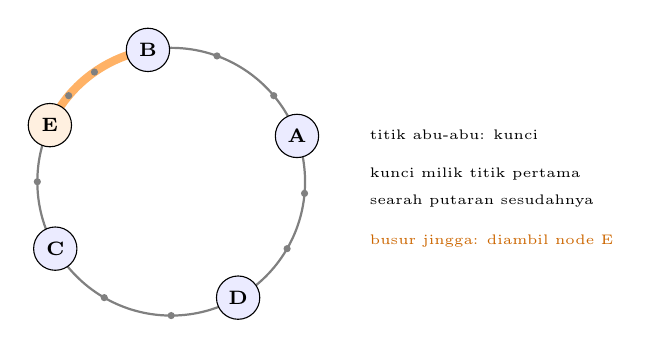
\begin{tikzpicture}[
    font=\scriptsize,
    titik/.style={circle, draw, minimum size=0.55cm, inner sep=0pt, font=\scriptsize\bfseries},
    panah/.style={-{Stealth[length=2mm]}, thick}
  ]
    \draw[thick, gray] (0,0) circle (1.7cm);
    \draw[line width=3pt, orange!60] (100:1.7cm) arc (100:155:1.7cm);
    \node[titik, fill=blue!8] at (20:1.7cm) {A};
    \node[titik, fill=blue!8] at (100:1.7cm) {B};
    \node[titik, fill=blue!8] at (210:1.7cm) {C};
    \node[titik, fill=blue!8] at (300:1.7cm) {D};
    \node[titik, fill=orange!12] at (155:1.7cm) {E};
    \foreach \sudut in {40, 70, 125, 140, 180, 240, 270, 330, 355} {
      \fill[gray] (\sudut:1.7cm) circle (1.3pt);
    }
    \node[font=\tiny, align=left, anchor=west] at (2.4,0.6) {titik abu-abu: kunci};
    \node[font=\tiny, align=left, anchor=west] at (2.4,0.1) {kunci milik titik pertama};
    \node[font=\tiny, align=left, anchor=west] at (2.4,-0.25) {searah putaran sesudahnya};
    \node[font=\tiny, align=left, anchor=west, orange!80!black] at (2.4,-0.75) {busur jingga: diambil node E};
  \end{tikzpicture}
  \caption{Lingkaran hash: \textit{node} baru E hanya mengambil kunci di busur
           sebelum titiknya}
  \label{fig:lingkaran14}
\end{figure}

Listing \ref{lst:petakan14} memperlihatkan kedua cara dalam satu fungsi.
Titik tiap \textit{node} pada lingkaran, yang sering disebut \textit{virtual node},
dihitung dari nomor \textit{node} dan nomor titiknya saja, sehingga menambah \textit{node}
tidak menggeser titik milik \textit{node} lama.

\begin{lstlisting}[style=PythonStyle, caption={Modulo dan \textit{consistent hashing} dalam satu fungsi, tersedia di \berkas{sources/chapter14/partisi.py}}, label={lst:petakan14}]
def petakan(cara, jumlah_node, daftar_nilai):
  """Mengembalikan nomor node untuk tiap kunci menurut satu cara pembagian."""
  if cara["jenis"] == "modulo":
    return [nilai % jumlah_node for nilai in daftar_nilai]
  posisi, pemilik = buat_lingkaran(jumlah_node, cara["titik_per_node"])
  return [pemilik[bisect.bisect_right(posisi, nilai) % len(posisi)]
          for nilai in daftar_nilai]
\end{lstlisting}

Tabel \ref{tab:partisi14} memuat hasilnya untuk 100.000 kunci pelanggan yang
dibagi ke empat \textit{node}, lalu ke lima \textit{node}. Kolom terberat menurut permintaan
memakai sebaran Zipf: pelanggan peringkat pertama datang dua kali lebih sering
daripada peringkat kedua, tiga kali lebih sering daripada peringkat ketiga,
dan seterusnya.

\begin{table}[!htb]
  \centering
  \caption{Empat \textit{node} menjadi lima, idealnya 20\% kunci pindah dan 20\% tiap
           \textit{node}, hasil perhitungan nyata}
  \label{tab:partisi14}
  \begin{tabularx}{\textwidth}{Xlll}
    \hline
    \textbf{Cara} & \textbf{Kunci pindah} & \textbf{Terberat, kunci} & \textbf{Terberat, permintaan} \\
    \hline
    modulo & 80,2\% & 20,2\% & 24,3\% \\
    \hline
    \textit{consistent hashing}, 1 titik & 2,1\% & 49,2\% & 43,3\% \\
    \hline
    \textit{consistent hashing}, 100 titik & 20,2\% & 21,2\% & 26,9\% \\
    \hline
  \end{tabularx}
\end{table}

Dua contoh dari tabel itu:
\begin{enumerate}
  \item Modulo memindahkan 80,2\% kunci untuk satu \textit{node} tambahan. Pada data
        sebesar 500 GB, itu berarti sekitar 400 GB disalin lewat jaringan,
        sementara sistemnya tetap harus melayani.
  \item \textit{Consistent hashing} dengan 100 titik per \textit{node} memindahkan
        20,2\%, hampir persis angka idealnya, dan \textit{node} terberatnya hanya
        memegang 21,2\% kunci.
\end{enumerate}

Baris tengah memuat kejanggalan. Satu titik per \textit{node} hanya memindahkan 2,1\%
kunci, jauh di bawah ideal, dan angka sekecil itu justru tanda buruk. Titik
tunggal \textit{node} baru kebetulan jatuh di busur yang sempit, sehingga \textit{node} itu
hampir tidak membawa kunci apa pun, sedangkan satu \textit{node} lama tetap memegang
49,2\% kunci. Banyak titik per \textit{node} meratakan panjang busur, dan karena
itulah \textit{virtual node} dipakai.

Kolom terakhir memperlihatkan batas partisi. Pembagian yang rata menurut
kunci belum tentu rata menurut beban. Pelanggan teratas pada sebaran Zipf ini
sendirian membawa sekitar 8,3\% seluruh permintaan, sehingga \textit{node} yang
memegangnya mencapai 24,3\% sampai 26,9\%, berapa pun cara bagi yang dipakai.
Kunci panas seperti itu diredam dengan \textit{cache} dan replika baca, bukan
dengan cara membagi kunci.

Pertanyaan berikutnya, berapa replika, replika baca, dan \textit{shard} yang
dibutuhkan untuk beban 100 kali lipat. Jawabannya disusun per layanan, karena
tiap layanan tumbuh dan dibatasi oleh hal yang berbeda. Listing
\ref{lst:rencana14} memperlihatkan inti perhitungannya.

\begin{lstlisting}[style=PythonStyle, caption={Replika, \textit{shard}, dan replika baca dari angka terukur, tersedia di \berkas{sources/chapter14/rencana-kapasitas.py}}, label={lst:rencana14}]
  replika = math.ceil(target_rps / budget_replika_rps)
  shard = max(1, math.ceil(tulis_qps / budget_node_qps))
  replika_baca_per_shard = math.ceil(baca_qps / shard / budget_node_qps)
  node_basis_data = shard * (1 + replika_baca_per_shard)
\end{lstlisting}

Tiap \textit{budget} hanya 60\% dari kapasitas terukur. Sisanya adalah ruang
untuk lonjakan dan untuk \textit{node} yang \textit{down}, sehingga rencananya tidak bergantung
pada keadaan yang serba lancar. Kapasitas satu replika, 106,8 permintaan per
detik, dan kapasitas satu \textit{node} basis data, 198,2 \textit{query} per detik,
diambil dari Tabel \ref{tab:skala14}. Biaya per \textit{node} hanyalah asumsi contoh,
bukan harga penyedia mana pun. Tabel \ref{tab:rencana14} memuat hasilnya.

\begin{table}[!htb]
  \centering
  \caption{Rencana kapasitas untuk beban 100 kali lipat, dihitung dari angka
           terukur dan asumsi biaya}
  \label{tab:rencana14}
  \begin{tabularx}{\textwidth}{Xllllll}
    \hline
    \textbf{Layanan} & \textbf{Target/s} & \textbf{Replika} & \textbf{Baca/s} & \textbf{Tulis/s} & \textbf{\textit{Node} basis data} & \textbf{Juta Rp} \\
    \hline
    katalog & 1.200 & 19 & 235,2 & 48,0 & 3 & 9,3 \\
    \hline
    pesanan & 300 & 5 & 360,0 & 540,0 & 10 & 13,5 \\
    \hline
    akun & 200 & 4 & 90,0 & 20,0 & 2 & 3,6 \\
    \hline
    \textbf{Jumlah} & & \textbf{28} & & & \textbf{15} & \textbf{26,4} \\
    \hline
  \end{tabularx}
\end{table}

Tabel itu punya dua konsekuensi praktis. Pertama, layanan pesanan membutuhkan
lima \textit{shard} walaupun bebannya seperempat beban katalog, karena 540
tulisan per detik melebihi \textit{budget} satu \textit{node}, yaitu 118,9. Kedua,
katalog cukup dengan tiga \textit{node} basis data karena 90\% bacaannya dijawab
\textit{cache}. Tanpa \textit{cache} itu, katalog membutuhkan 21 \textit{node}, dan
biaya bulanannya naik dari Rp 26,4 juta menjadi Rp 48,0 juta.

Satu batas lagi diperiksa rencana ini, yaitu koneksi. Tiap replika membuka
\textit{pool} berisi empat koneksi ke tiap \textit{node} layanannya, sehingga 19
replika katalog membuka 76 koneksi ke satu \textit{node}. Angka itu masih di bawah
batas 100. Pada beban 200 kali lipat, jumlahnya menjadi 152, dan di sanalah
\textit{connection pooler} seperti PgBouncer dari Bab 3 dibutuhkan
\cite{pgbouncer-features}.

\section{Sistem Multi-Region dan Edge Computing}

Sistem \textit{multi-region} dijalankan di beberapa wilayah geografis
sekaligus. Alasannya tiga: pengguna yang jauh dilayani dari tempat yang
dekat, satu wilayah yang padam tidak mematikan seluruh sistem, dan sebagian
data wajib disimpan di wilayah tertentu. Ketiganya dibayar dengan replikasi
data antarwilayah, yang lambat karena jaraknya.

Jarak itu tidak dapat ditawar dengan kode. Cahaya di dalam serat optik
merambat sekitar 200.000 kilometer per detik \cite{grigorik2013hpbn},
sehingga satu perjalanan bolak-balik, atau Round-Trip Time (RTT), sejauh
1.000 kilometer memakan sedikitnya 10 milidetik. Satu sambungan HTTP terenkripsi
yang baru membutuhkan sedikitnya tiga perjalanan bolak-balik sebelum byte pertama tiba:
jabat tangan TCP, jabat tangan Transport Layer Security (TLS) 1.3
\cite{rfc8446}, lalu permintaan HTTP itu sendiri.

Tabel \ref{tab:region14} menghitung batas bawah itu dari Jakarta ke empat
wilayah pusat data yang lazim dipakai.

\begin{table}[!htb]
  \centering
  \caption{Batas bawah waktu dari Jakarta, dihitung dari jarak lingkaran besar
           dan kecepatan cahaya di serat optik}
  \label{tab:region14}
  \begin{tabularx}{\textwidth}{Xlll}
    \hline
    \textbf{Wilayah server} & \textbf{Jarak} & \textbf{RTT minimum} & \textbf{Tiga RTT} \\
    \hline
    Singapura & 905 km & 9,1 ms & 27,2 ms \\
    \hline
    Tokyo & 5.782 km & 57,8 ms & 173,5 ms \\
    \hline
    Frankfurt & 11.119 km & 111,2 ms & 333,6 ms \\
    \hline
    Virginia, Amerika Serikat & 16.338 km & 163,4 ms & 490,1 ms \\
    \hline
  \end{tabularx}
\end{table}

Angka sungguhan selalu lebih besar daripada tabel itu, karena kabelnya tidak
lurus dan tiap perangkat di tengah jalan menambah waktu. Dua contoh kasus
nyata:
\begin{enumerate}
  \item Pengguna di Jakarta yang dilayani dari Singapura menunggu sedikitnya
        27,2 milidetik sebelum byte pertama. Angka itu kecil dibanding waktu
        server menyusun halamannya.
  \item Pengguna yang sama, bila dilayani dari Virginia, menunggu sedikitnya
        490,1 milidetik sebelum server mengerjakan apa pun. Tidak ada
        optimasi kode yang dapat mengembalikan setengah detik itu.
\end{enumerate}

Analoginya seperti gudang cabang. Toko yang hanya punya gudang pusat di
Jakarta mengirim lambat ke pelanggan di Papua. Gudang cabang mempercepat
pengiriman, tetapi stoknya kini tersebar, dan jumlah stok di tiap cabang harus
dicocokkan. Sebagian barang bahkan tidak boleh keluar dari wilayahnya sama
sekali.

Barang yang tidak boleh keluar itu nyata pada data pribadi. Undang-Undang
Nomor 27 Tahun 2022 tentang Pelindungan Data Pribadi (UU PDP) mengatur syarat
pengiriman data pribadi ke luar wilayah hukum Indonesia \cite{uu-pdp-2022}.
Karena itu rancangan \textit{multi-region} dimulai dengan memilah data:
katalog boleh disalin ke mana saja, sedangkan data pembeli disimpan di
wilayah yang diizinkan, lalu permintaan yang menyentuhnya diarahkan ke sana.

\textit{Edge computing} membawa sebagian kode lebih dekat lagi, yaitu ke
lokasi Content Delivery Network (CDN) di dekat pengguna, seperti pada
perbandingan \textit{edge} dan \textit{origin} di Bab 8. Agar dapat berjalan
di ratusan lokasi dengan murah, kodenya dijalankan di lingkungan yang ringan.
Dokumentasi Cloudflare menyebut satu \textit{isolate} dapat dinyalakan
sekitar seratus kali lebih cepat daripada satu proses Node.js di dalam
\textit{container} atau mesin virtual \cite{cloudflare-workers}.

Batasnya ada pada data. Fungsi di \textit{edge} yang membutuhkan basis data
di Virginia tetap membayar 163,4 milidetik tiap pertanyaan ke sana. Karena
itu yang pantas dikerjakan di \textit{edge} adalah pekerjaan yang tidak
membutuhkan basis data pusat: mengarahkan permintaan, memeriksa token,
menyajikan \textit{cache}, atau menyesuaikan halaman dari isi cookie.

\section{Progressive Web App dan Offline-First}

PWA adalah aplikasi web yang dapat dipasang seperti aplikasi biasa dan tetap
bekerja ketika jaringannya buruk. Dua bagian membuatnya begitu. Manifest
menjelaskan nama, ikon, dan alamat awal aplikasinya \cite{w3c-appmanifest}.
\textit{Service worker} adalah skrip yang berdiri di antara halaman dan
jaringan, menangkap tiap permintaan halaman, lalu memutuskan apakah
\textit{response}-nya diambil dari jaringan atau dari \textit{cache} miliknya
sendiri
\cite{w3c-service-workers}.

Analoginya seperti petugas loket perpustakaan yang menyimpan \textit{copy} daftar
buku di laci. Ketika sistem pusat \textit{down}, petugas tetap dapat menunjukkan daftar
terakhir, lengkap dengan tanggal \textit{copy}-nya, alih-alih menyuruh mahasiswa
pulang. Mahasiswa yang belum pernah datang, sayangnya, tidak punya \textit{copy}
apa pun di laci itu.

\textit{Offline-first} melangkah lebih jauh. Aplikasinya bekerja lebih dahulu
dengan data di perangkat, lalu menyelaraskannya dengan server ketika jaringan
tersedia \cite{kleppmann2019localfirst}. Demo bab ini memakai bentuk yang
paling sederhana, yaitu membaca saat \textit{offline}. Menulis saat
\textit{offline} menambah satu masalah lagi, yaitu \textit{conflict} ketika
dua perangkat mengubah data yang sama sebelum sempat diselaraskan.

Gambar \ref{fig:sw14} memperlihatkan dua aturan yang dipakai \textit{service
worker} demo bab ini.

\begin{figure}[!htb]
  \centering
  \begin{tikzpicture}[
    font=\scriptsize,
    kotak/.style={draw, rounded corners, minimum height=0.8cm,
                  minimum width=2.1cm, align=center, font=\scriptsize\bfseries},
    panah/.style={-{Stealth[length=2mm]}, thick}
  ]
    \node[kotak, fill=blue!8] (halaman) at (0,0) {Halaman\\{\tiny\mdseries aplikasi.js}};
    \node[kotak, fill=praditagreen!15, minimum height=1.6cm] (sw) at (3.4,0) {Service\\worker\\{\tiny\mdseries sw.js}};
    \node[kotak, fill=green!10] (cache) at (8.6,0.9) {Cache\\{\tiny\mdseries katalog-v1}};
    \node[kotak, fill=orange!12] (server) at (8.6,-0.9) {Server\\{\tiny\mdseries port 8120}};

    \draw[panah] (halaman) -- node[font=\tiny, above] {fetch} (sw);
    \draw[panah] (sw.east) -- ++(0.3,0) |- node[font=\tiny, above, pos=0.7] {kerangka: \textit{cache} dulu} (cache.west);
    \draw[panah] (sw.east) -- ++(0.3,0) |- node[font=\tiny, below, pos=0.7] {data: jaringan dulu} (server.west);
    \draw[panah, dashed] (server.north) -- node[font=\tiny, right] {disimpan} (cache.south);
  \end{tikzpicture}
  \caption{Kerangka halaman diambil dari \textit{cache} lebih dahulu, data
           katalog dari jaringan lebih dahulu}
  \label{fig:sw14}
\end{figure}

Aturan untuk data tertulis pada Listing \ref{lst:sw14}. Tiap \textit{response}
yang berhasil disimpan, sehingga \textit{copy} di \textit{cache} selalu yang terakhir
dilihat pengguna. Ketika jaringannya gagal, \textit{copy} itu dipakai dan diberi
penanda, agar halaman tahu datanya bukan data baru.

\begin{lstlisting}[language=TypeScript, caption={Jaringan lebih dahulu, \textit{copy} terakhir bila gagal, tersedia di \berkas{sources/chapter14/statis/sw.js}}, label={lst:sw14}]
async function jaringanLebihDahulu(permintaan) {
  const cache = await caches.open(NAMA_CACHE);
  try {
    const respon = await fetch(permintaan);
    await cache.put(permintaan, respon.clone());
    return respon;
  } catch (gagal) {
    const tersimpan = await cache.match(permintaan);
    if (!tersimpan) {
      throw gagal;
    }
    return tandaiDariCache(tersimpan);
  }
}
\end{lstlisting}

Pengukurannya membuat empat kunjungan, masing-masing dengan proses Chrome
baru, seperti browser yang ditutup lalu dibuka lagi. Chrome dikendalikan
lewat Chrome DevTools Protocol, sehingga alat ukur menunggu sampai
\textit{service worker} benar-benar siap, bukan menebak lamanya. Tabel
\ref{tab:offline14} memuat hasilnya.

\begin{table}[!htb]
  \centering
  \caption{Empat kunjungan ke katalog PWA, dua di antaranya ketika server
           \textit{down}, hasil pengukuran nyata}
  \label{tab:offline14}
  \begin{tabularx}{\textwidth}{Xlllll}
    \hline
    \textbf{Kunjungan} & \textbf{Server} & \textbf{Buku} & \textbf{Sumber} & \textbf{Tampil ms} & \textbf{Ke server} \\
    \hline
    1, profil baru & hidup & 8 & jaringan & 377 & 11 \\
    \hline
    2, profil sama & hidup & 8 & jaringan & 62 & 2 \\
    \hline
    3, profil sama & \textit{down} & 8 & \textit{cache} & 31 & 0 \\
    \hline
    4, profil baru & \textit{down} & 0 & gagal & - & 0 \\
    \hline
  \end{tabularx}
\end{table}

Dua contoh dari tabel itu:
\begin{enumerate}
  \item Pada kunjungan ketiga servernya sudah \textit{down}, tetapi delapan buku tetap
        tampil dalam 31 milidetik, dan tidak satu permintaan pun sampai ke
        server. Seluruh halaman dan datanya datang dari \textit{cache}.
  \item Pada kunjungan keempat servernya sama-sama \textit{down}, tetapi profilnya
        baru. Chrome melaporkan \texttt{net::ERR\_CONNECTION\_REFUSED}, dan
        tidak ada buku yang tampil. \textit{Service worker} hanya melindungi
        pengguna yang pernah datang.
\end{enumerate}

Kunjungan pertama justru yang paling mahal, dengan 11 permintaan. Halaman
memuat dirinya sekali, lalu \textit{service worker} yang baru terpasang
memuat ulang seluruh kerangka untuk disimpan. Angka 377 milidetik pada baris
itu juga memuat biaya profil browser yang baru dibuat, sehingga tidak
seluruhnya akibat jaringan.

Baris kedua memuat kejanggalan. Halamannya sudah dikendalikan
\textit{service worker}, tetapi dua permintaan masih sampai ke server. Yang
pertama data katalog, dan itu memang aturannya. Yang kedua permintaan
navigasi ke \texttt{/}, padahal kerangka dilayani dari \textit{cache}.
Permintaan itu dikirim Chrome sendiri bersamaan dengan menyalakan
\textit{service worker}, agar tidak perlu menunggu bila \textit{service
worker}-nya ternyata meneruskan ke jaringan. Karena \textit{service worker}
menjawab dari \textit{cache}, \textit{response} dari jaringan itu dibuang. Permintaan itu
hilang ketika Chrome dijalankan dengan
\texttt{--disable-features=ServiceWorkerAutoPreload}, dan hanya permintaan
data yang tersisa.

Aturan ini punya dua konsekuensi praktis. Pertama, data dari \textit{cache}
wajib diberi tahu umurnya, sehingga halaman demo menulis jam pembuatan
datanya, bukan berpura-pura data itu baru. Kedua, isi \textit{cache} harus
diberi versi. Nama \texttt{katalog-v1} dinaikkan setiap kerangka berubah, dan
\textit{cache} versi lama dihapus ketika \textit{service worker} baru aktif.
Tanpa itu, pengguna terjebak pada kerangka lama yang tidak pernah diganti.

\section{WebAssembly dan Serverless}

WebAssembly, disingkat Wasm, adalah format biner yang dijalankan browser di
dalam \textit{sandbox} yang sama dengan JavaScript, dengan kecepatan yang
mendekati kode asli mesin \cite{haas2017wasm}. Kode Wasm umumnya hasil
kompilasi bahasa lain, misalnya C, C++, atau Rust, sehingga pustaka yang
sudah ada dapat dibawa ke browser tanpa ditulis ulang
\cite{w3c-wasm-core}.

Wasm bukan pengganti JavaScript. Ia tidak menyentuh Document Object Model
(DOM) secara langsung, sehingga tiap perubahan tampilan tetap lewat
JavaScript, dan tiap perpindahan antara keduanya ada biayanya. Tabel
\ref{tab:wasm14} merangkum kapan Wasm layak dipakai.

\begin{table}[!htb]
  \centering
  \caption{Kapan WebAssembly layak dipakai pada aplikasi web}
  \label{tab:wasm14}
  \begin{tabularx}{\textwidth}{XX}
    \hline
    \textbf{Layak} & \textbf{Tidak layak} \\
    \hline
    perhitungan berat di browser, misalnya pengolahan gambar atau video & mengubah DOM, mengisi form, menangani klik \\
    \hline
    membawa pustaka C, C++, atau Rust yang sudah teruji & logika bisnis yang cukup ditulis dengan JavaScript \\
    \hline
    pekerjaan yang sama di browser dan di server & halaman yang harus tampil secepat mungkin pada kunjungan pertama \\
    \hline
  \end{tabularx}
\end{table}

Baris terakhir perlu penjelasan. Modul Wasm harus diunduh dan dikompilasi
sebelum dipakai, sehingga modul berukuran beberapa megabyte menambah waktu
pada kunjungan pertama, persis seperti \textit{bundle} JavaScript yang besar
pada Bab 5.

\textit{Serverless} memindahkan urusan server ke penyedia. Pengembang hanya
menulis satu fungsi, penyedia menyalakannya ketika ada permintaan,
menambah \textit{copy}-nya ketika permintaan bertambah, mematikannya ketika sepi,
lalu menagih per panggilan \cite{jonas2019serverless}. Harganya adalah
\textit{cold start}: panggilan pertama pada \textit{copy} yang baru harus
menunggu lingkungannya dinyalakan, sedangkan panggilan berikutnya pada
\textit{copy} yang sama, disebut \textit{warm}, langsung dikerjakan
\cite{aws-lambda-lifecycle}.

Analoginya seperti laboratorium komputer yang dimatikan ketika kosong.
Mahasiswa pertama yang datang menunggu komputer menyala dan programnya
terbuka. Mahasiswa sesudahnya langsung bekerja, selama komputernya belum
dimatikan lagi.

Fungsi demo bab ini menghitung ongkos kirim, seperti pada Listing
\ref{lst:fungsi14}. Bentuknya bentuk \textit{handler} \textit{serverless}:
menerima satu peristiwa, mengembalikan satu hasil, dan tidak menyimpan apa
pun di antara dua panggilan.

\begin{lstlisting}[style=PythonStyle, caption={Satu \textit{handler} tanpa \textit{state}, tersedia di \berkas{sources/chapter14/fungsi.py}}, label={lst:fungsi14}]
def tangani(peristiwa):
  """Menghitung ongkos kirim satu paket. Bentuknya seperti handler serverless.

  Handler hanya menerima peristiwa dan mengembalikan hasil. Ia tidak
  menyimpan apa pun di antara dua pemanggilan, karena pemanggilan berikutnya
  belum tentu sampai ke proses yang sama.
  """
  kilogram = math.ceil(peristiwa["berat_gram"] / GRAM_PER_KILOGRAM)
  tarif = TARIF_PER_KILOGRAM_RUPIAH.get(peristiwa["kota"],
                                        TARIF_BAWAAN_RUPIAH)
  return {"ongkir_rupiah": kilogram * tarif}
\end{lstlisting}

Tabel \ref{tab:coldstart14} membandingkan tiga cara memanggil fungsi yang
sama. \textit{Warm} memakai satu proses yang terus hidup. \textit{Cold start}
menyalakan proses baru untuk tiap panggilan. Varian ketiga ditambah memuat
sepuluh modul pustaka standar saat proses dinyalakan, menirukan fungsi yang
membawa dependensi.

\begin{table}[!htb]
  \centering
  \caption{Satu fungsi yang sama dengan tiga cara memanggil, hasil
           pengukuran nyata}
  \label{tab:coldstart14}
  \begin{tabularx}{\textwidth}{Xlll}
    \hline
    \textbf{Cara} & \textbf{p50 ms} & \textbf{p95 ms} & \textbf{Kali lipat} \\
    \hline
    \textit{warm}, proses dipakai ulang & 0,012 & 0,012 & 1 \\
    \hline
    \textit{cold start} & 19,069 & 22,248 & 1.610 \\
    \hline
    \textit{cold start}, dengan dependensi & 105,565 & 118,585 & 8.911 \\
    \hline
  \end{tabularx}
\end{table}

Dua contoh dari tabel itu:
\begin{enumerate}
  \item Fungsi yang sama memakan 0,012 milidetik ketika \textit{warm} dan
        19,069 milidetik ketika \textit{cold start}. Seluruh selisihnya adalah
        menyalakan interpreter, bukan menghitung ongkos kirim.
  \item Sepuluh modul tambahan menaikkan \textit{cold start} menjadi 105,565
        milidetik. Dependensi dibayar pada tiap \textit{cold start}, bukan
        sekali saja.
\end{enumerate}

Angka itu baru bagian yang ditentukan kode fungsinya. Layanan
\textit{serverless} sungguhan masih menambahkan waktu mengunduh kode dan
menyalakan lingkungannya. Firecracker, mesin virtual ringan di balik Amazon
Web Services (AWS) Lambda, dilaporkan menyala dalam waktu sekitar 125 milidetik
\cite{agache2020firecracker}.

Aturan ini punya dua konsekuensi praktis. Pertama, pekerjaan persiapan,
misalnya membuka koneksi basis data, ditaruh di luar \textit{handler},
karena bagian itu dikerjakan sekali per lingkungan lalu dipakai ulang pada
tiap panggilan \textit{warm} \cite{aws-lambda-lifecycle}. Kedua, fungsi
yang diskalakan menjadi ratusan \textit{copy} dapat membuka ratusan koneksi
sekaligus ke satu basis data \cite{aws-lambda-concurrency}, sehingga
\textit{pool} atau \textit{connection pooler} dari Bab 3 tetap dibutuhkan,
justru lebih mendesak.

\section{Aplikasi Web Terintegrasi Large Language Model}

Fitur berbantuan LLM memanggil sebuah model bahasa lewat Application
Programming Interface (API) milik penyedianya. Model menghasilkan jawaban
token demi token, dan tiap token dibayar. Tiga hal mengikuti dari sifat itu:
jawabannya lambat dalam hitungan detik, biayanya tumbuh bersama jumlah
pemakaian, dan isi pertanyaannya keluar dari sistem sendiri menuju
penyedia.

Analoginya seperti konsultasi dengan dosen pembimbing yang sibuk. Tiap
pertanyaan memakan waktu dan, pada penyedia model, memakan biaya.
\textit{Streaming} berarti dosennya mulai menjelaskan begitu paham
pertanyaannya, bukan menulis surat lengkap lebih dahulu. \textit{Cache}
kecocokan persis seperti lembar tanya-jawab yang ditempel di pintu: hanya
menolong bila pertanyaannya ditulis persis sama.

Gambar \ref{fig:llm14} memperlihatkan susunannya. Browser tidak pernah
berbicara langsung dengan model. Ia bertanya ke server sendiri, dan server
itulah yang memegang kunci API. Jawabannya kembali ke browser sebagai
Server-Sent Events (SSE), seperti pada Bab 13.

\begin{figure}[!htb]
  \centering
  \begin{tikzpicture}[
    font=\scriptsize,
    kotak/.style={draw, rounded corners, minimum height=0.9cm,
                  minimum width=2.2cm, align=center, font=\scriptsize\bfseries},
    panah/.style={-{Stealth[length=2mm]}, thick}
  ]
    \node[kotak, fill=blue!8] (browser) at (0,0) {Browser\\{\tiny\mdseries tanpa kunci API}};
    \node[kotak, fill=praditagreen!15, minimum height=1.3cm] (asisten) at (4.7,0) {Asisten\\{\tiny\mdseries kunci API, \textit{cache}}\\{\tiny\mdseries port 8121}};
    \node[kotak, fill=orange!12] (model) at (9.2,0) {Model tiruan\\{\tiny\mdseries port 8122}};

    \draw[panah] ([yshift=0.2cm]browser.east) -- node[font=\tiny, above] {pertanyaan} ([yshift=0.2cm]asisten.west);
    \draw[panah] ([yshift=-0.2cm]asisten.west) -- node[font=\tiny, below] {token demi token, SSE} ([yshift=-0.2cm]browser.east);
    \draw[panah] ([yshift=0.2cm]asisten.east) -- node[font=\tiny, above] {+ kunci API} ([yshift=0.2cm]model.west);
    \draw[panah] ([yshift=-0.2cm]model.west) -- node[font=\tiny, below] {token, lalu biaya} ([yshift=-0.2cm]asisten.east);
  \end{tikzpicture}
  \caption{Fitur berbantuan LLM di sisi server: kunci API dan pencatatan
           biaya berada di satu tempat}
  \label{fig:llm14}
\end{figure}

Listing \ref{lst:kunci14} memperlihatkan tempat kunci itu ditambahkan. Kunci
dibaca dari \textit{environment} proses server, seperti \textit{secret} pada
Bab 7, dan tidak pernah ikut terkirim ke browser.

\begin{lstlisting}[style=PythonStyle, caption={Kunci API ditambahkan di sisi server, tersedia di \berkas{sources/chapter14/asisten.py}}, label={lst:kunci14}]
def tanya_model(pertanyaan, stream):
  """Mengirim pertanyaan ke model beserta kunci API, mengembalikan response.

  Kunci API hanya ada di environment proses ini. Ia ditambahkan di sini,
  pada sisi server, sehingga tidak pernah ikut terkirim ke browser.
  """
  koneksi = HTTPConnection(HOST, PORT_MODEL, timeout=BATAS_WAKTU_DETIK)
  badan = json.dumps({"pertanyaan": pertanyaan, "stream": stream}).encode()
  koneksi.request("POST", "/v1/jawab", body=badan, headers={
      "Authorization": f"Bearer {KUNCI_MODEL}",
      "Content-Type": JENIS_ISI_JSON,
      "Content-Length": str(len(badan)),
  })
  return koneksi.getresponse()
\end{lstlisting}

Modelnya tiruan, dan itu disengaja. Token pertamanya keluar sesudah 0,6
detik, lalu 120 token menyusul tiap 20 milidetik. Angka itu ditetapkan di
\berkas{model-tiruan.py}, bukan diukur dari model mana pun, sehingga yang
terukur adalah akibat rancangan aplikasinya, bukan kecepatan modelnya.
Jawabannya dialirkan ke browser sebagai SSE, token demi token. Tabel \ref{tab:llm14} memuat empat skenario yang diukur dari
sisi browser.

\begin{table}[!htb]
  \centering
  \caption{Empat skenario pertanyaan pada model dengan waktu yang ditetapkan,
           hasil pengukuran nyata}
  \label{tab:llm14}
  \begin{tabularx}{\textwidth}{Xllll}
    \hline
    \textbf{Skenario} & \textbf{Token pertama ms} & \textbf{Selesai ms} & \textbf{Token dibayar} & \textbf{Cache} \\
    \hline
    tanpa \textit{streaming} & 2.983,8 & 2.983,8 & 126 & MISS \\
    \hline
    \textit{streaming} & 601,7 & 3.003,4 & 127 & MISS \\
    \hline
    \textit{streaming}, kalimat sama & 0,7 & 0,7 & 0 & HIT \\
    \hline
    \textit{streaming}, kalimat lain & 602,0 & 3.000,2 & 127 & MISS \\
    \hline
  \end{tabularx}
\end{table}

Dua contoh dari tabel itu:
\begin{enumerate}
  \item \textit{Streaming} memajukan token pertama dari 2.983,8 menjadi 601,7
        milidetik, tetapi jawaban tetap selesai pada 3.003,4 milidetik.
        \textit{Streaming} menyembunyikan \textit{latency}, tidak
        menghapusnya, dan biaya tokennya tetap dibayar penuh.
  \item Pertanyaan yang sama persis dijawab \textit{cache} dalam 0,7
        milidetik tanpa satu token pun. Pertanyaan yang maknanya sama tetapi
        kalimatnya lain kembali membayar 127 token, karena \textit{cache}
        kecocokan persis tidak mengenali makna.
\end{enumerate}

Baris terakhir itulah alasan \textit{semantic cache} dijadikan topik
penelitian keempat di \texttt{README.md}: pertanyaan dicocokkan menurut
maknanya, lalu diverifikasi sebelum jawabannya dipakai ulang, karena jawaban
untuk pertanyaan yang mirip belum tentu benar untuk pertanyaan yang lain.

Biayanya mudah dihitung dari kolom token. Dengan 127 token per pertanyaan,
10.000 pertanyaan sehari berarti 1,27 juta token sehari, dan harganya tinggal
dikalikan dengan tarif penyedia yang berlaku. Tarif itu berubah dan berbeda
antarpenyedia, sehingga \textit{budget} token per pengguna dan
\textit{rate limiting} dari Bab 12 lebih dapat diandalkan daripada perkiraan
tarif.

Masalah yang paling berat justru bukan waktu atau biaya, melainkan keamanan
dan privasi. Model menerima perintah dan data dalam satu teks yang sama,
sehingga data dapat menyamar sebagai perintah. Tabel \ref{tab:risikollm14}
memuat lima risiko dari daftar OWASP yang paling dekat dengan aplikasi web
\cite{owasp-llm-top10}.

\begin{table}[!htb]
  \centering
  \caption{Lima risiko aplikasi LLM menurut OWASP, beserta cara meredamnya
           pada aplikasi web}
  \label{tab:risikollm14}
  \begin{tabularx}{\textwidth}{lX}
    \hline
    \textbf{Risiko} & \textbf{Cara meredam} \\
    \hline
    LLM01 Prompt Injection & pisahkan perintah dari data, dan anggap teks dari pengguna atau dokumen sebagai data, bukan perintah \\
    \hline
    LLM02 Sensitive Information Disclosure & jangan kirim data pribadi yang tidak dibutuhkan, dan periksa aturan penyimpanan data penyedia \\
    \hline
    LLM05 Improper Output Handling & perlakukan jawaban model seperti masukan pengguna: di-\textit{escape} dan ditampilkan lewat \texttt{textContent} \\
    \hline
    LLM06 Excessive Agency & beri model hak sekecil mungkin, dan minta persetujuan pengguna sebelum tindakan yang mengubah data \\
    \hline
    LLM10 Unbounded Consumption & batasi token per permintaan dan per pengguna, lalu pasang \textit{rate limiting} \\
    \hline
  \end{tabularx}
\end{table}

Baris ketiga mengulang pelajaran Bab 7 dengan pelaku baru. Jawaban model
dapat berisi HyperText Markup Language (HTML) atau skrip, entah karena
modelnya keliru atau karena pertanyaannya sengaja disusun begitu. Memasukkan
jawaban itu lewat \texttt{innerHTML} sama dengan membuka pintu
Cross-Site Scripting (XSS). Baris kedua mengulang pelajaran seksi
\textit{multi-region}: data pribadi yang dikirim ke penyedia di luar negeri
tunduk pada aturan UU PDP \cite{uu-pdp-2022}.

\section{Ringkasan}

Penskalaan horizontal bekerja selama pekerjaannya ada di replika. Dari satu
ke dua replika, \textit{throughput} naik dari 106,8 menjadi 186,6 permintaan
per detik. Sesudah itu basis data berkapasitas 200 \textit{query} per detik
menjadi \textit{bottleneck}, dan empat maupun delapan replika berhenti di
198,2 dan 198,0. Ketika basis datanya dibesarkan menjadi 16 koneksi, delapan
replika mencapai 347,8 permintaan per detik dengan efisiensi 41\%, karena
\textit{bottleneck}-nya pindah ke komputer itu sendiri.

Memecah aplikasi menjadi layanan menambah biaya pada tiap panggilan.
Sepuluh panggilan harga memakan 0,0012 milidetik sebagai fungsi dan 1,4436
milidetik lewat HTTP, lebih dari seribu kali lipat, bahkan di 127.0.0.1.
Imbalannya adalah layanan yang di-\textit{deploy} dan diskalakan sendiri,
sehingga pemecahan pantas dilakukan hanya ketika ada alasan yang terukur.

Membagi data pun ada harganya. Ketika empat \textit{node} ditambah satu, modulo
memindahkan 80,2\% kunci, sedangkan \textit{consistent hashing} dengan 100
titik per \textit{node} memindahkan 20,2\%. Satu titik per \textit{node} tampak lebih hemat
dengan 2,1\%, tetapi membiarkan satu \textit{node} memegang 49,2\% kunci. Rencana
kapasitas untuk beban 100 kali lipat membutuhkan 28 replika dan 15 \textit{node} basis
data, dengan lima \textit{shard} untuk pesanan karena tulisannya tidak dapat
dibagi ke replika baca, sedangkan \textit{cache} katalog menghemat 18 \textit{node}.

Teknologi yang sedang tumbuh memindahkan masalah yang sama ke tempat baru.
\textit{Service worker} menampilkan delapan buku dalam 31 milidetik ketika
server \textit{down}, tetapi hanya bagi pengguna yang pernah datang. \textit{Cold
start} memakan 19,069 milidetik, lebih dari seribu kali panggilan
\textit{warm}, dan 105,565 milidetik dengan dependensi. \textit{Streaming}
LLM memajukan token pertama dari 2.983,8 menjadi 601,7 milidetik tanpa
memajukan selesainya, dan \textit{cache} kecocokan persis tidak mengenali
kalimat lain yang bermakna sama. Jarak pun tidak dapat ditawar: 490,1
milidetik sebelum byte pertama dari Jakarta ke Virginia.

Pesan utama bab ini adalah bahwa tiap teknik penskalaan memindahkan
\textit{bottleneck}, tidak menghapusnya. Rencana yang baik menyebutkan di
mana \textit{bottleneck} berikutnya akan muncul, berapa biaya
memindahkannya, dan angka mana yang membuktikannya.

\section{Latihan}

Seluruh file yang dipakai pada latihan ini tersedia di
\berkas{sources/chapter14/}, dihitung relatif terhadap akar repositori.
Latihan ini hanya membutuhkan Python 3 dan Google Chrome atau Chromium, tanpa
Docker dan tanpa pustaka tambahan. Skrip pengukur menyalakan dan mematikan
sendiri proses yang diukurnya.

\berkas{ukur-skala.py} sengaja membebani, tetapi yang dibebaninya hanya
proses yang dinyalakannya sendiri di 127.0.0.1. Seluruh alat ukur lain
bersifat mengamati. Angka \textit{throughput} bergantung pada jumlah \textit{core} dan
batas daya komputer, sehingga hasil tiap mahasiswa akan berbeda,
sedangkan pola perbandingannya akan sama. Angka pada bab ini diukur dengan
Python 3.15 dan Chrome 157 pada laptop Intel Core i9-11900H.

Sebelum mulai, periksa kedua perkakasnya seperti pada Listing
\ref{lst:c14-siapkan}. \textit{Sanity check} ini mencegah pengukuran yang
gagal di tengah jalan karena Chrome tidak ditemukan.

\begin{lstlisting}[language=bash, caption={Memeriksa perkakas latihan, dijalankan dari \berkas{sources/chapter14/}}, label={lst:c14-siapkan}]
cd sources/chapter14
python3 --version
google-chrome --version

# Keluarannya:
# Python 3.15.2
# Google Chrome 157.0.8103.38
\end{lstlisting}

\subsection*{Latihan 1: Penskalaan Horizontal dan Bottleneck yang Pindah}

Latihan ini membuktikan bahwa menambah replika berhenti menolong ketika
komponen bersamanya penuh, lalu memperlihatkan \textit{bottleneck} pindah
ketika komponen itu dibesarkan.

\begin{enumerate}
  \item Jalankan \berkas{ukur-skala.py}, seperti pada Listing
        \ref{lst:c14-lat1-jalan}, lalu catat keempat barisnya.
  \item Kalikan \textit{throughput} dengan p50 dalam detik pada tiap baris,
        lalu bandingkan hasilnya dengan jumlah \textit{worker}, yaitu 32.
  \item Jalankan ulang dengan \texttt{JUMLAH\_KONEKSI=16} di depan
        perintahnya, lalu catat keempat barisnya.
  \item Isi Tabel \ref{tab:c14-lat1-hasil}. Tabel \ref{tab:c14-lat1-contoh}
        memperlihatkan contoh yang sudah terisi.
  \item Jawab tiga pertanyaan berikut. Pertama, mengapa empat dan delapan
        replika berhenti pada angka yang hampir sama dengan empat koneksi?
        Kedua, mengapa p50 empat dan delapan replika sama persis, padahal
        replikanya berlipat? Ketiga, mengapa delapan replika dengan 16
        koneksi hanya mencapai efisiensi sekitar 40\%, dan apa yang berubah
        bila tiap replika berjalan di mesin terpisah?
\end{enumerate}

\begin{lstlisting}[language=bash, caption={Mengukur penskalaan dengan dua kapasitas basis data, tersedia di \berkas{sources/chapter14/ukur-skala.py}}, label={lst:c14-lat1-jalan}]
python3 ukur-skala.py
JUMLAH_KONEKSI=16 python3 ukur-skala.py

# Keluarannya, baris tabel saja, 4 koneksi lalu 16 koneksi:
#   Replika  Permintaan/detik   p50 ms   p95 ms  Efisiensi
#         1             106.8    286.1    547.5       100%
#         2             186.6    161.4    278.3        87%
#         4             198.2    161.4    168.6        46%
#         8             198.0    161.4    168.9        23%
#
#         1             105.0    288.9    581.5       100%
#         2             179.8    169.5    302.2        86%
#         4             285.0    105.2    181.5        68%
#         8             347.8     87.4    143.3        41%
\end{lstlisting}

\begin{table}[!htb]
  \centering
  \caption{Contoh hasil Latihan 1 yang sudah terisi}
  \label{tab:c14-lat1-contoh}
  \begin{tabularx}{\textwidth}{Xlll}
    \hline
    \textbf{Replika} & \textbf{4 koneksi, per detik} & \textbf{16 koneksi, per detik} & \textbf{16 koneksi, efisiensi} \\
    \hline
    1 & 106,8 & 105,0 & 100\% \\
    \hline
    2 & 186,6 & 179,8 & 86\% \\
    \hline
    4 & 198,2 & 285,0 & 68\% \\
    \hline
    8 & 198,0 & 347,8 & 41\% \\
    \hline
  \end{tabularx}
\end{table}

\begin{table}[!htb]
  \centering
  \caption{Lembar isian hasil pengukuran Latihan 1}
  \label{tab:c14-lat1-hasil}
  \begin{tabularx}{\textwidth}{Xlll}
    \hline
    \textbf{Replika} & \textbf{4 koneksi, per detik} & \textbf{16 koneksi, per detik} & \textbf{16 koneksi, efisiensi} \\
    \hline
    1 & \dots & \dots & \dots \\
    \hline
    2 & \dots & \dots & \dots \\
    \hline
    4 & \dots & \dots & \dots \\
    \hline
    8 & \dots & \dots & \dots \\
    \hline
  \end{tabularx}
\end{table}

\subsection*{Latihan 2: Partisi Data dan Kunci yang Pindah}

Latihan ini membuktikan bahwa cara membagi data menentukan berapa banyak data
yang harus disalin ketika \textit{node} ditambah, dan bahwa angka yang kecil belum
tentu baik.

\begin{enumerate}
  \item Jalankan \berkas{partisi.py}, seperti pada Listing
        \ref{lst:c14-lat2-jalan}, lalu catat ketiga barisnya.
  \item Ubah \texttt{JUMLAH\_NODE\_AKHIR} di \berkas{partisi.py} menjadi 8,
        jalankan ulang, lalu catat kolom kunci pindahnya.
  \item Kembalikan \texttt{JUMLAH\_NODE\_AKHIR} menjadi 5.
  \item Isi Tabel \ref{tab:c14-lat2-hasil}. Tabel \ref{tab:c14-lat2-contoh}
        memperlihatkan contoh yang sudah terisi.
  \item Jawab tiga pertanyaan berikut. Pertama, mengapa modulo dari empat ke
        delapan \textit{node} hanya memindahkan 50,0\% kunci, jauh lebih sedikit
        daripada dari empat ke lima? Kedua, mengapa satu titik per \textit{node} yang
        hanya memindahkan 2,1\% kunci justru tanda buruk? Ketiga, mengapa
        \textit{node} terberat menurut permintaan selalu lebih berat daripada menurut
        kunci, berapa pun cara baginya?
\end{enumerate}

\begin{lstlisting}[language=bash, caption={Membandingkan dua cara membagi data, tersedia di \berkas{sources/chapter14/partisi.py}}, label={lst:c14-lat2-jalan}]
python3 partisi.py

# Keluarannya:
#   100000 kunci, 4 node menjadi 5 node, ideal 20.0% tiap node
#
#   Cara                           Pindah Terberat, kunci Terberat, permintaan
#   modulo                          80.2%           20.2%                24.3%
#   consistent hashing, 1 titik      2.1%           49.2%                43.3%
#   consistent hashing, 100 titik   20.2%           21.2%                26.9%
#
# Dengan JUMLAH_NODE_AKHIR = 8, tiga baris tabelnya:
#   modulo                          50.0%           12.6%                20.9%
#   consistent hashing, 1 titik     43.4%           27.7%                24.0%
#   consistent hashing, 100 titik   49.5%           13.7%                20.5%
\end{lstlisting}

\begin{table}[!htb]
  \centering
  \caption{Contoh hasil Latihan 2 yang sudah terisi}
  \label{tab:c14-lat2-contoh}
  \begin{tabularx}{\textwidth}{Xlll}
    \hline
    \textbf{Cara} & \textbf{Pindah, 4 ke 5} & \textbf{Pindah, 4 ke 8} & \textbf{Terberat, 4 ke 5} \\
    \hline
    modulo & 80,2\% & 50,0\% & 20,2\% \\
    \hline
    \textit{consistent hashing}, 1 titik & 2,1\% & 43,4\% & 49,2\% \\
    \hline
    \textit{consistent hashing}, 100 titik & 20,2\% & 49,5\% & 21,2\% \\
    \hline
  \end{tabularx}
\end{table}

\begin{table}[!htb]
  \centering
  \caption{Lembar isian hasil perhitungan Latihan 2}
  \label{tab:c14-lat2-hasil}
  \begin{tabularx}{\textwidth}{Xlll}
    \hline
    \textbf{Cara} & \textbf{Pindah, 4 ke 5} & \textbf{Pindah, 4 ke 8} & \textbf{Terberat, 4 ke 5} \\
    \hline
    modulo & \dots & \dots & \dots \\
    \hline
    \textit{consistent hashing}, 1 titik & \dots & \dots & \dots \\
    \hline
    \textit{consistent hashing}, 100 titik & \dots & \dots & \dots \\
    \hline
  \end{tabularx}
\end{table}

Angka pada latihan ini dihitung, bukan diukur dengan jam, sehingga akan sama
persis pada komputer mana pun. Yang dilaporkan tetap pola perbandingannya,
karena angka itulah yang menjadi dasar memilih cara bagi.

\subsection*{Latihan 3: Rencana Kapasitas untuk Beban 100 Kali Lipat}

Latihan ini menyusun rencana penskalaan dari angka hasil pengukuran sendiri,
lalu memperlihatkan komponen mana yang paling mahal dan mana yang pertama kali
melewati batas.

\begin{enumerate}
  \item Isi \texttt{kapasitas\_replika\_rps} di \berkas{rencana.json} dengan
        \textit{throughput} satu replika dari Latihan 1, dan
        \texttt{kapasitas\_node\_basis\_data\_qps} dengan
        \textit{throughput} empat replika pada empat koneksi.
  \item Jalankan \berkas{rencana-kapasitas.py}, seperti pada Listing
        \ref{lst:c14-lat3-jalan}, lalu catat baris totalnya.
  \item Ubah \texttt{hit\_ratio\_cache} katalog menjadi 0,0, jalankan ulang,
        catat totalnya, lalu kembalikan menjadi 0,9.
  \item Ubah \texttt{kelipatan\_beban} menjadi 200, jalankan ulang, catat
        pemeriksaan koneksi yang gagal, lalu kembalikan menjadi 100.
  \item Isi Tabel \ref{tab:c14-lat3-hasil}. Tabel \ref{tab:c14-lat3-contoh}
        memperlihatkan contoh yang sudah terisi.
  \item Jawab tiga pertanyaan berikut. Pertama, mengapa pesanan membutuhkan
        lima \textit{shard} sedangkan katalog cukup satu, padahal beban
        katalog empat kali lebih besar? Kedua, berapa \textit{node} basis data dan
        berapa rupiah per bulan yang dihemat \textit{cache} katalog? Ketiga,
        pada beban 200 kali lipat, batas apa yang pertama kali terlewati, dan
        komponen apa yang menjawabnya?
\end{enumerate}

\begin{lstlisting}[language=bash, caption={Menyusun rencana kapasitas, tersedia di \berkas{sources/chapter14/rencana-kapasitas.py}}, label={lst:c14-lat3-jalan}]
python3 rencana-kapasitas.py

# Keluarannya:
#   Beban 100 kali lipat, utilisasi maksimum 60%
#
#   Layanan   Target Replika  Baca/s Tulis/s Shard Node BD Juta Rp
#   katalog     1200      19   235.2    48.0     1       3     9.3
#   pesanan      300       5   360.0   540.0     5      10    13.5
#   akun         200       4    90.0    20.0     1       2     3.6
#
#   katalog     76 koneksi per node basis data, batas 100: aman
#   pesanan     20 koneksi per node basis data, batas 100: aman
#   akun        16 koneksi per node basis data, batas 100: aman
#
#   Total: 28 replika, 15 node basis data, Rp 26.4 juta per bulan
\end{lstlisting}

\begin{table}[!htb]
  \centering
  \caption{Contoh hasil Latihan 3 yang sudah terisi}
  \label{tab:c14-lat3-contoh}
  \begin{tabularx}{\textwidth}{Xllll}
    \hline
    \textbf{Skenario} & \textbf{Replika} & \textbf{\textit{Node} basis data} & \textbf{Juta Rp} & \textbf{Koneksi katalog} \\
    \hline
    100 kali, \textit{cache} 90\% & 28 & 15 & 26,4 & 76, aman \\
    \hline
    100 kali, tanpa \textit{cache} katalog & 28 & 33 & 48,0 & 76, aman \\
    \hline
    200 kali, \textit{cache} 90\% & 55 & 28 & 50,1 & 152, perlu \textit{pooler} \\
    \hline
  \end{tabularx}
\end{table}

\begin{table}[!htb]
  \centering
  \caption{Lembar isian hasil perhitungan Latihan 3}
  \label{tab:c14-lat3-hasil}
  \begin{tabularx}{\textwidth}{Xllll}
    \hline
    \textbf{Skenario} & \textbf{Replika} & \textbf{\textit{Node} basis data} & \textbf{Juta Rp} & \textbf{Koneksi katalog} \\
    \hline
    100 kali, \textit{cache} 90\% & \dots & \dots & \dots & \dots \\
    \hline
    100 kali, tanpa \textit{cache} katalog & \dots & \dots & \dots & \dots \\
    \hline
    200 kali, \textit{cache} 90\% & \dots & \dots & \dots & \dots \\
    \hline
  \end{tabularx}
\end{table}

Biaya pada rencana ini hanyalah asumsi contoh yang tertulis di
\berkas{rencana.json}. Yang dinilai adalah susunan dan alasannya: layanan
mana yang membutuhkan \textit{shard}, berapa yang dihemat \textit{cache}, dan
batas mana yang terlewati lebih dahulu.

\subsection*{Latihan 4: Mode Offline Progressive Web App}

Latihan ini membuktikan bahwa halaman yang dilindungi \textit{service worker}
tetap tampil ketika servernya \textit{down}, dan bahwa perlindungan itu hanya berlaku
bagi pengguna yang pernah datang.

\begin{enumerate}
  \item Jalankan \berkas{ukur-offline.py}, seperti pada Listing
        \ref{lst:c14-lat4-jalan}, lalu catat keempat barisnya.
  \item Cocokkan jumlah permintaan kunjungan pertama dengan isi
        \texttt{KERANGKA} di \berkas{statis/sw.js}.
  \item Nyalakan \texttt{python3 aplikasi.py}, buka
        \texttt{http://127.0.0.1:8120/} di Chrome dua kali, lalu periksa
        bagian Application di DevTools: \textit{service worker}-nya dan isi
        \textit{cache} \texttt{katalog-v1}.
  \item Matikan \berkas{aplikasi.py}, muat ulang halamannya, lalu catat jam
        pembuatan data yang tertulis di atas daftar buku.
  \item Isi Tabel \ref{tab:c14-lat4-hasil}. Tabel \ref{tab:c14-lat4-contoh}
        memperlihatkan contoh yang sudah terisi.
  \item Jawab tiga pertanyaan berikut. Pertama, mengapa kunjungan pertama
        justru yang paling banyak mengirim permintaan? Kedua, kunjungan
        ketiga dan keempat sama-sama tanpa server, apa yang membuat hasilnya
        berbeda? Ketiga, apa yang wajib diperlihatkan halaman kepada pengguna
        ketika datanya berasal dari \textit{cache}?
\end{enumerate}

\begin{lstlisting}[language=bash, caption={Empat kunjungan dengan Chrome tanpa jendela, tersedia di \berkas{sources/chapter14/ukur-offline.py}}, label={lst:c14-lat4-jalan}]
python3 ukur-offline.py

# Keluarannya:
#   Kunjungan       Server Buku  Sumber    Saat mulai    Tampil ms Ke server
#   1, profil baru  hidup     8  jaringan  belum               377        11
#   2, profil sama  hidup     8  jaringan  mengendalikan        62         2
#   3, profil sama  down      8  cache     mengendalikan        31         0
#   4, profil baru  down      0  gagal     -                     -         0
#                   Chrome: net::ERR_CONNECTION_REFUSED
\end{lstlisting}

\begin{table}[!htb]
  \centering
  \caption{Contoh hasil Latihan 4 yang sudah terisi}
  \label{tab:c14-lat4-contoh}
  \begin{tabularx}{\textwidth}{Xllll}
    \hline
    \textbf{Kunjungan} & \textbf{Server} & \textbf{Buku} & \textbf{Sumber} & \textbf{Ke server} \\
    \hline
    1, profil baru & hidup & 8 & jaringan & 11 \\
    \hline
    2, profil sama & hidup & 8 & jaringan & 2 \\
    \hline
    3, profil sama & \textit{down} & 8 & \textit{cache} & 0 \\
    \hline
    4, profil baru & \textit{down} & 0 & gagal & 0 \\
    \hline
  \end{tabularx}
\end{table}

\begin{table}[!htb]
  \centering
  \caption{Lembar isian hasil pengamatan Latihan 4}
  \label{tab:c14-lat4-hasil}
  \begin{tabularx}{\textwidth}{Xllll}
    \hline
    \textbf{Kunjungan} & \textbf{Server} & \textbf{Buku} & \textbf{Sumber} & \textbf{Ke server} \\
    \hline
    1, profil baru & hidup & \dots & \dots & \dots \\
    \hline
    2, profil sama & hidup & \dots & \dots & \dots \\
    \hline
    3, profil sama & \textit{down} & \dots & \dots & \dots \\
    \hline
    4, profil baru & \textit{down} & \dots & \dots & \dots \\
    \hline
  \end{tabularx}
\end{table}

Jumlah permintaan pada kunjungan kedua bergantung pada versi Chrome. Chrome
157 yang dipakai pada bab ini mengirim satu permintaan navigasi bersamaan
dengan menyalakan \textit{service worker}, sehingga hasilnya dua, bukan satu.
Browser lain atau versi lain dapat mencatat angka berbeda, sedangkan pola
kunjungan ketiga dan keempat akan sama.

\subsection*{Latihan 5: Cold Start Fungsi Serverless}

Latihan ini membuktikan bahwa \textit{cold start} ditentukan oleh apa yang
dimuat sebelum fungsinya dipanggil, bukan oleh fungsinya sendiri.

\begin{enumerate}
  \item Jalankan \berkas{ukur-cold-start.py}, seperti pada Listing
        \ref{lst:c14-lat5-jalan}, lalu catat ketiga barisnya.
  \item Tambahkan \texttt{"multiprocessing"}, \texttt{"ssl"}, dan
        \texttt{"difflib"} ke \texttt{DAFTAR\_DEPENDENSI} di
        \berkas{fungsi.py}, jalankan ulang, lalu catat baris ketiganya.
  \item Kembalikan \texttt{DAFTAR\_DEPENDENSI} seperti semula.
  \item Isi Tabel \ref{tab:c14-lat5-hasil}. Tabel \ref{tab:c14-lat5-contoh}
        memperlihatkan contoh yang sudah terisi.
  \item Jawab tiga pertanyaan berikut. Pertama, mengapa \textit{cold start}
        lebih dari seribu kali panggilan \textit{warm}, padahal fungsinya
        sama? Kedua, bagian mana dari \textit{cold start} layanan
        \textit{serverless} sungguhan yang tidak terukur di sini? Ketiga,
        mengapa pekerjaan persiapan seperti membuka koneksi basis data
        sebaiknya ditaruh di luar \textit{handler}?
\end{enumerate}

\begin{lstlisting}[language=bash, caption={Membandingkan \textit{warm} dan \textit{cold start}, tersedia di \berkas{sources/chapter14/ukur-cold-start.py}}, label={lst:c14-lat5-jalan}]
python3 ukur-cold-start.py

# Keluarannya:
#   Cara                             p50 ms   p95 ms  Kali lipat
#   warm, proses dipakai ulang        0.012    0.012           1
#   cold start                       19.069   22.248        1610
#   cold start, dengan dependensi   105.565  118.585        8911
#
# Baris ketiga dengan tiga dependensi tambahan:
#   cold start, dengan dependensi   111.941  123.417        8583
\end{lstlisting}

\begin{table}[!htb]
  \centering
  \caption{Contoh hasil Latihan 5 yang sudah terisi}
  \label{tab:c14-lat5-contoh}
  \begin{tabularx}{\textwidth}{Xlll}
    \hline
    \textbf{Cara} & \textbf{p50 ms} & \textbf{p95 ms} & \textbf{Kali lipat} \\
    \hline
    \textit{warm} & 0,012 & 0,012 & 1 \\
    \hline
    \textit{cold start} & 19,069 & 22,248 & 1.610 \\
    \hline
    \textit{cold start}, 10 dependensi & 105,565 & 118,585 & 8.911 \\
    \hline
    \textit{cold start}, 13 dependensi & 111,941 & 123,417 & 8.583 \\
    \hline
  \end{tabularx}
\end{table}

\begin{table}[!htb]
  \centering
  \caption{Lembar isian hasil pengukuran Latihan 5}
  \label{tab:c14-lat5-hasil}
  \begin{tabularx}{\textwidth}{Xlll}
    \hline
    \textbf{Cara} & \textbf{p50 ms} & \textbf{p95 ms} & \textbf{Kali lipat} \\
    \hline
    \textit{warm} & \dots & \dots & \dots \\
    \hline
    \textit{cold start} & \dots & \dots & \dots \\
    \hline
    \textit{cold start}, 10 dependensi & \dots & \dots & \dots \\
    \hline
    \textit{cold start}, 13 dependensi & \dots & \dots & \dots \\
    \hline
  \end{tabularx}
\end{table}

Baris terakhir contoh memuat kejanggalan. Tiga dependensi tambahan menaikkan
p50 menjadi 111,941 milidetik, tetapi kolom kali lipatnya justru turun dari
8.911 menjadi 8.583. Kedua baris berasal dari dua kali jalan yang berbeda,
dan pembaginya, yaitu p50 \textit{warm}, naik dari 0,012 menjadi 0,013
milidetik pada jalan kedua. Penyebut yang sekecil itu membuat kolom kali
lipat tidak dapat dibandingkan antarjalan, sehingga yang dibandingkan adalah
kolom milidetiknya.
